\documentclass[a4paper,12pt,UTF8]{ctexart}

% if you need to pass options to natbib, use, e.g.:
\PassOptionsToPackage{numbers, compress}{natbib}
% before loading nips_2016
%
% to avoid loading the natbib package, add option nonatbib:
% \usepackage[nonatbib]{nips_2016}

%\usepackage{nips_2016}

% to compile a camera-ready version, add the [final] option, e.g.:
\usepackage[final]{finalreport}

\usepackage[utf8]{inputenc} % allow utf-8 input
\usepackage[T1]{fontenc}    % use 8-bit T1 fonts
\usepackage{hyperref}       % hyperlinks
\usepackage{url}            % simple URL typesetting
\usepackage{booktabs}       % professional-quality tables
\usepackage{amsfonts}       % blackboard math symbols
\usepackage{nicefrac}       % compact symbols for 1/2, etc.
\usepackage{microtype}      % microtypography
\usepackage{CJKutf8}
\usepackage{graphicx}
\usepackage{amsmath}
\usepackage{pdfpages}
\usepackage{titlesec}
\usepackage{indentfirst}

\setlength{\parindent}{2em}

\newcommand{\norm}[1]{\left\lVert#1\right\rVert}

\title{《人工神经网络》大作业最终报告:神经图像编辑}


% The \author macro works with any number of authors. There are two
% commands used to separate the names and addresses of multiple
% authors: \And and \AND.
%
% Using \And between authors leaves it to LaTeX to determine where to
% break the lines. Using \AND forces a line break at that point. So,
% if LaTeX puts 3 of 4 authors names on the first line, and the last
% on the second line, try using \AND instead of \And before the third
% author name.

\newcommand{\song}{\CJKfamily{zhsong}}	% 宋体
\newcommand{\hei}{\CJKfamily{zhhei}}	% 黑体
\newcommand{\fs}{\CJKfamily{zhfs}}		% 仿宋
\newcommand{\kai}{\CJKfamily{zhkai}}	% 楷体
\newcommand{\li}{\CJKfamily{zhli}}		% 隶书
\newcommand{\you}{\CJKfamily{zhyou}}	% 幼圆

\author{
  徐鉴劲 \\
  2015011313 \\
  计算机科学与技术系 \\
  清华大学 \\
  \texttt{xujj15@mails.tsinghua.edu.cn}
  %% examples of more authors
  \AND
  贾越凯 \\
  2015011335 \\
  计算机科学与技术系 \\
  清华大学 \\
  \texttt{jiayk15@mails.tsinghua.edu.cn} \\
  \AND
  寇明阳 \\
  2015011318 \\
  计算机科学与技术系 \\
  清华大学 \\
  \texttt{kmy15@mails.tsinghua.edu.cn} \\
  %% \And
  %% Coauthor \\
  %% Affiliation \\
  %% Address \\
  %% \texttt{email} \\
}

\begin{document}

\maketitle

\begin{abstract}

\end{abstract}


\section{引言}

本项目神经图像编辑项目,是通过简笔画生成图像、编辑已有的图像。

% 更多简介与导引 -- 【徐鉴劲】

项目的成果主要有以下部分:

\begin{enumerate}
\item 成功复现了高质量的动漫人物头像生成网络。
\item 成功应用编辑图像方法于极深层的神经网络。
\item 获得了高于基线的生成成果和编辑成果。包括生成真实度上升,生成清晰度上升($64 \times 64 \Rightarrow 128 \times 128$)和肉眼可见的编辑质量上升
\item 基于Web/Server的交互界面。
\end{enumerate}

\section{相关工作}

% --- 所有 --【徐鉴劲】

\section{方法}

\subsection{框架}

我们的项目分为两个阶段实现,第一阶段不编辑一个给定的具体图像,先考虑编辑一个随机生成的图像,如图 \ref{fig:workflow1};第二阶段再加入一个编码网络来完成对于具体图像的编辑,在图 \ref{fig:workflow2} 中进行了说明。

\begin{figure}
  \centering
  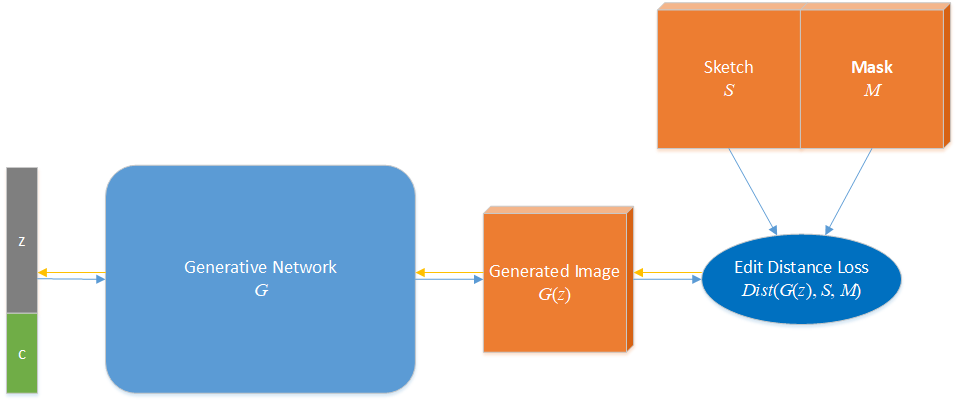
\includegraphics[width=1\linewidth]{figs/workflow1.png}
  \caption{\kai 第一阶段的项目解决方法。从随机向量出发,由生成网络生成初始结果,用户给定简笔画和对应的遮罩,由编辑距离函数计算误差和倒数,并借此更新 $z$,达到编辑图像的目的。蓝箭头表示数据流向,橙色箭头表示导数。}
  \label{fig:workflow1}
\end{figure}

\begin{figure}
  \centering
  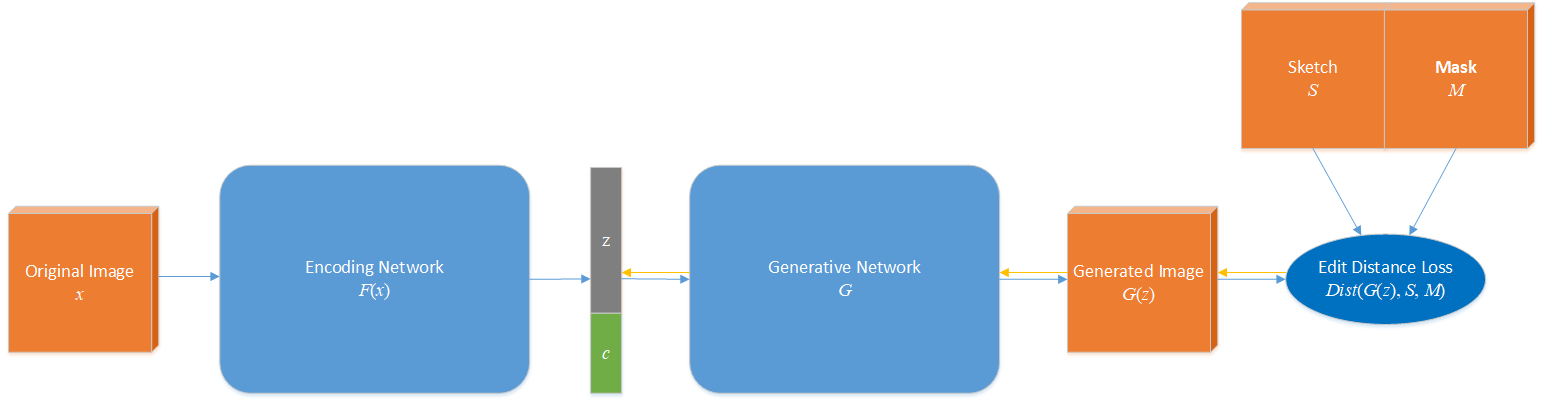
\includegraphics[width=1\linewidth]{figs/workflow2.png}
  \caption{\kai 第二阶段的项目解决方法。从一个待编辑图像出发,先通过编码网络生成 $z$ 与 $c$,然后经过生成网络生成重构结果,用户给定简笔画和对应的遮罩,由编辑距离函数计算误差和导数,并借此更新 $z$,达到编辑图像的目的。蓝箭头表示数据流向,橙色箭头表示导数。}
  \label{fig:workflow2}
\end{figure}

\subsection{编辑图像}

一个生成网络$G(z, c)$接受随机向量$z$(遵循高斯分布)和条件向量$c$作为输入,生成图像$I = G(z, c)$。同时用户给定编辑图像$I'$,例如一副简笔画,则可以据此给出生成图像与编辑图像之间的距离$Dist(G(z, c), I')$。设$I$在像素点$(i, j)$处的RGB颜色向量为$I_{ij}$。定义

\begin{equation}
  M_{ij} =
  \begin{cases}
    [0, 0, 0]   &  \text{if $\norm{I'_{ij}} = 0$} \\
    [1, 1, 1]   &  \text{if $\norm{I'_{ij}} \neq 0$}
  \end{cases}
\end{equation}

则有

\begin{equation}
  Dist(I, I') = \frac{\sum_{ij} |I_{ij} - I'_{ij}| \cdot M_{ij}}{1 + \sum_{ij} M_{ij}}
\end{equation}

假设 $G$ 已经得到,本文的基本目标是求使$Dist(G(z, c), I')$最小的$z$和$c$:

\begin{equation}
  \arg\min_{z, c} Dist(G(z, c), I')
\end{equation}

设学习率为$lr$。为求这样的$z$和$c$,先给出随机的合法初值$z_{0}$和$c_{0}$,再将距离函数对$z_{0}$和$c_{0}$求偏导:

\begin{equation}
  \Delta z_{0} = \frac{\partial}{\partial z} Dist(G(z_{0}, c_{0}), I')
\end{equation}
\begin{equation}
  \Delta c_{0} = \frac{\partial}{\partial c} Dist(G(z_{0}, c_{0}), I')
\end{equation}

之后,在$z$和$c$的反函数域上以学习率$lr$使用Gradient Descent算法进行学习,并限制$\tilde z_{1}$和$\tilde c_{1}$在合法的边界中:
\begin{equation}
  \tilde z_{1} = arc \tanh z_{0} - lr \cdot \Delta z_{0}
\end{equation}

\begin{equation}
  \tilde c_{1} = - \log (\frac{1}{c_{0}} - 1) - lr \cdot \Delta c_{0}
\end{equation}

最后,将$\tilde z_{1}$和$\tilde c_{1}$变换为原来的函数域,得到新的值$z_{1}$和$c_{1}$:

\begin{equation}
  z_{1} = \tanh (\tilde z_{1})
\end{equation}
\begin{equation}
  c_{1} = [ sigmoid(\tilde c_{1}) ]
\end{equation}

重复这样的学习,即可使$Dist(G(z, c), I')$不断减小,直到生成符合要求的图片。
% --- 剩余所有部分 -- 【寇明扬】

\subsection{训练网络}

% --- 训练设置 -- 【xjj】

设真实数据集为$D_R$,一个训练样例可以表示成$x \sim P_r$,同时随机向量 $z$ 和 $c$ 有$z \sim P_z$和$c \sim P_c$。构造一个判别网络$D(I)$。

\begin{equation}
  \min_{\theta_G,\theta_f} \max_{\theta_D} \mathbb{E}_{(x, z, c) \sim (P_r, P_z, P_c)} \Big[ \log D(x) + \log\big(1 - D(G(z, c))\big) + \log\big(1 - D(G(f(x)))\big)\Big]
\end{equation}

进一步地,使用DRAGAN~\cite{kodali2017convergence}替代普通的GAN训练:

\begin{equation}
\begin{aligned}
  \mathcal{L}_{adv}(D) &= -\mathbb{E}_{x\sim P_{data}}[\log D(x)] - \mathbb{E}_{x\sim P_{noise},c\sim P_{cond}}\big[\log(1-D(G(z,c)))\big] \\
  \mathcal{L}_{cls}(D) &= \mathbb{E}_{x\sim P_{data}}\big[\log P_D[label_x|x]\big] + \mathbb{E}_{x\sim P_{noise},c\sim P_{cond}}\Big[\log\big(P_D[c|G(z,c)]\big)\Big] \\
  \mathcal{L}_{gp}(D) &= \mathbb{E}_{\tilde{x}\sim P_{perturebed\_data}}\left[\big(\norm{\nabla_{\tilde{x}}D(\tilde{x})}_2-1\big)^2\right] \\
  \mathcal{L}_{adv}(G) &= \mathbb{E}_{x\sim P_{noise},c\sim P_{cond}}\big[\log D(G(z,c))\big] \\
  \mathcal{L}_{cls}(G) &= \mathbb{E}_{x\sim P_{noise},c\sim P_{cond}}\big[\log P_D[c|G(z,c)]\big] \\
  \mathcal{L}(D) &= \mathcal{L}_{cls}(D) + \lambda_{adv}\mathcal{L}_{adv}(D)+ \lambda_{gp}\mathcal{L}_{gp}(D) \\
  \mathcal{L}(G) &= \lambda_{adv}\mathcal{L}_{adv}(G) + \mathcal{L}_{cls}(G)
\end{aligned}
\end{equation}

% -- 公式:将formule.png写成代码 -- 【jyk】

% -- deprecated begin

其中,$P_{cond}$ 表示给定标签下的先验分布;$\mathcal{L}_{adv}$,$\mathcal{L}_{gp}$ 和 $\mathcal{L}_{reg}$ 分别表示 adversarial,gradient penalty 和 weight regularization 的 loss。

\begin{equation}
\begin{aligned}
  \mathcal{L}_{reg} &= \norm{\theta_D}_2 + \norm{\theta_G}_2 \\
  \mathcal{L}_{gp} &= \norm{\left(\frac{\partial D(\tilde x)}{\partial \tilde x}\right)^2 - 1 }_2
\end{aligned}
\end{equation}

$\tilde x$表示了生成图像和真实图像的线性插值,$\alpha \in (0, 1)$是随机的插值系数。

\begin{equation}
  \tilde x = \alpha (x - G(z, c)) + G(z, c)
\end{equation}

% -- deprecated end

神经图像编辑的范围十分广阔,本项目研究动漫头像编辑这一子类上的应用。

\section{实验}

\subsection{生成对抗训练}

% -- MNIST --

% -- 训练设置 -- 【徐鉴劲】

% -- IAN与DRAGAN的对比 -- 【徐鉴劲】

% -- GETCHU -- 【徐鉴劲】

% -- DRAGAN网络的loss图、中间演变 -- 【徐鉴劲】

\subsection{图像编辑}

% -- 实际设置 -- 【寇明扬】

% -- 选几张展示编辑效果(参考ppt) -- 【寇明扬】

% -- 结论 -- 【寇明扬】

\subsection{前端}

% -- 有关前端的设置 -- 【贾越凯】

% -- 前端的性能 -- 【贾越凯】

% -- 前端的展示 -- 【贾越凯】

\section{结论}

% -- 总结 -- 【徐鉴劲】

% -- 个人收获 ---【寇明扬】 【贾越凯】

\section*{参考文献}

\medskip

{\small
\bibliographystyle{ieee}
\bibliography{egbib}
}

\end{document}
